\documentclass[12pt]{article}
\usepackage{lingmacros}
\usepackage{tree-dvips}
\usepackage{graphicx} %package to manage images
\usepackage{float}
\usepackage{subcaption}%package for enabling multiple images in a single figure
\graphicspath{ {/} }
\begin{document}

\section*{Creating a Grid and Graphical Representation}

Our grid relies on several key assumptions. Our grid always assumes that a grid is n x n, and that the start is always at the top left corner and the goal at the bottom right corner. Each tile of the grid has a number on it that respresents the number of tiles you can move in any direction form that grid. Every tile on a grid can go to at least one other tile on the grid.

\begin{figure}[H]
    \centering
    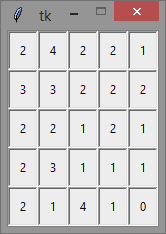
\includegraphics[width=0.3\linewidth]{basic_5x5_solvable}
    \caption{A 5x5 grid with a solution.}
    \label{fig:5x5_solution}
\end{figure}

\section*{Puzzle Evaluations}

In order to evaluate our generated puzzles, we implemented a Breadth First Search (BFS) algorithm equivalent to the one described in the task. Evaluated grids are filled with either numbers or X's that represent the number of moves to reach that cell or that a cell is unreachable, respectively. The bottom most and right hand most cell contains either the value of the puzzle or an X which indicates that the puzzle is not solvable. Below are examples of evaluated n x n grids for varying values of n (n = 5, 7, 9, 11) with their corresponding values and if they are solvable or not.

%5x5 Grids
%GOOD
\begin{figure}[H]
	\begin{subfigure}{.5\textwidth}
		\centering
     		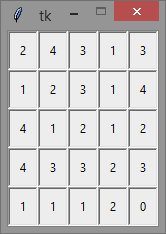
\includegraphics[width = .6\linewidth]{5x5_puzzle_3}
     		\caption{Puzzle}
     		\label{fig2:sfig1}
	\end{subfigure}
	\begin{subfigure}{.5\textwidth}
		\centering
		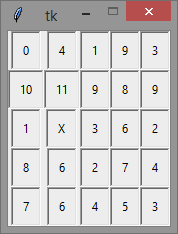
\includegraphics[width = .6\linewidth]{5x5_eval_3}
		\caption{Evaluation}
		\label{fig2:sfig2}
	\end{subfigure}
\caption{Solvable 5x5 puzzle. Value: 3.}
\label{fig:5x5good}
\end{figure}
%BAD
\begin{figure}[H]
	\begin{subfigure}{.5\textwidth}
		\centering
     		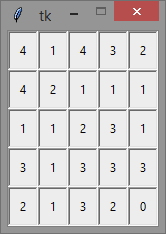
\includegraphics[width = .6\linewidth]{5x5_puzzle_-3}
     		\caption{Puzzle}
     		\label{fig3:sfig1}
	\end{subfigure}
	\begin{subfigure}{.5\textwidth}
		\centering
		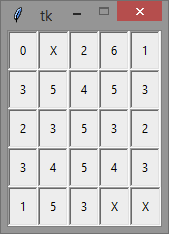
\includegraphics[width = .6\linewidth]{5x5_eval_-3}
		\caption{Evaluation}
		\label{fig3:sfig2}
	\end{subfigure}
\caption{Unsolvable 5x5 puzzle. Value: -3.}
\label{fig:5x5bad}
\end{figure}

%7x7 Grids
\begin{figure}[H]
	\begin{subfigure}{.5\textwidth}
		\centering
     		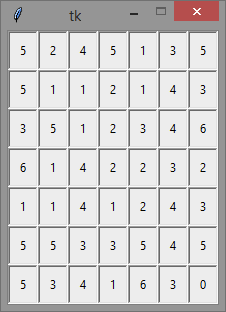
\includegraphics[width = .6\linewidth]{7x7_puzzle_5}
     		\caption{Puzzle}
     		\label{fig4:sfig1}
	\end{subfigure}
	\begin{subfigure}{.5\textwidth}
		\centering
		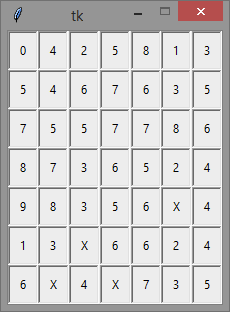
\includegraphics[width = .6\linewidth]{7x7_eval_5}
		\caption{Evaluation}
		\label{fig4:sfig2}
	\end{subfigure}
\caption{Solvable 7x7 puzzle. Value: 5.}
\label{fig:7x7good}
\end{figure}

\begin{figure}[H]
	\begin{subfigure}{.5\textwidth}
		\centering
     		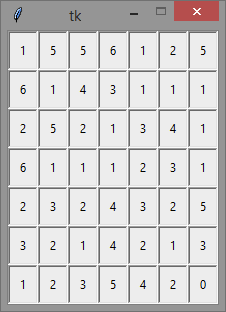
\includegraphics[width = .6\linewidth]{7x7_puzzle_-3}
     		\caption{Puzzle}
     		\label{fig5:sfig1}
	\end{subfigure}
	\begin{subfigure}{.5\textwidth}
		\centering
		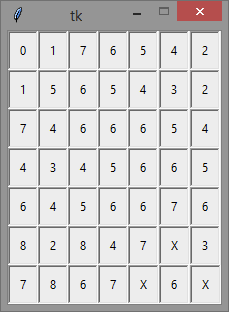
\includegraphics[width = .6\linewidth]{7x7_eval_-3}
		\caption{Evaluation}
		\label{fig5:sfig2}
	\end{subfigure}
\caption{Unsolvable 7x7 puzzle. Value: -3.}
\label{fig:7x7bad}
\end{figure}

%9x9 Grids
\begin{figure}[H]
	\begin{subfigure}{.5\textwidth}
		\centering
     		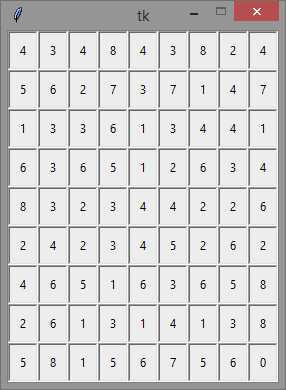
\includegraphics[width = .6\linewidth]{9x9_puzzle_8}
     		\caption{Puzzle}
     		\label{fig6:sfig1}
	\end{subfigure}
	\begin{subfigure}{.5\textwidth}
		\centering
		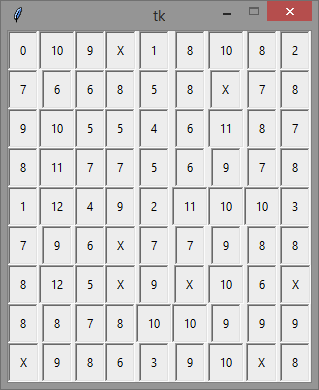
\includegraphics[width = .6\linewidth]{9x9_eval_8}
		\caption{Evaluation}
		\label{fig6:sfig2}
	\end{subfigure}
\caption{Solvable 9x9 puzzle. Value: 8.}
\label{fig:9x9good}
\end{figure}

\begin{figure}[H]
	\begin{subfigure}{.5\textwidth}
		\centering
     		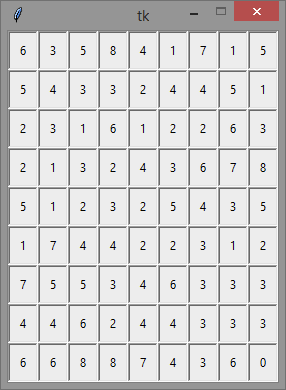
\includegraphics[width = .6\linewidth]{9x9_puzzle_-15}
     		\caption{Puzzle}
     		\label{fig7:sfig1}
	\end{subfigure}
	\begin{subfigure}{.5\textwidth}
		\centering
		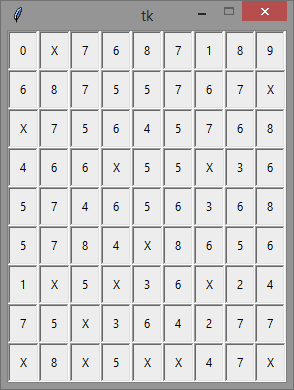
\includegraphics[width = .6\linewidth]{9x9_eval_-15}
		\caption{Evaluation}
		\label{fig7:sfig2}
	\end{subfigure}
\caption{Unsolvable 9x9 puzzle. Value: -15.}
\label{fig:9x9bad}
\end{figure}

%11x11 Grids
\begin{figure}[H]
	\begin{subfigure}{.5\textwidth}
		\centering
     		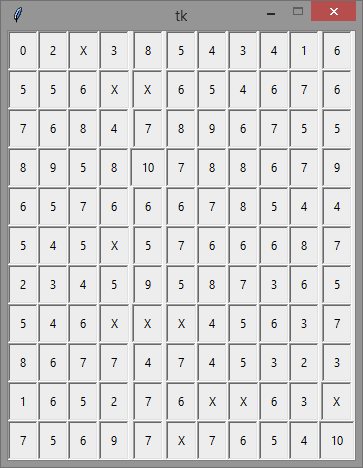
\includegraphics[width = .6\linewidth]{11x11_1_puzzle_10}
     		\caption{Puzzle}
     		\label{fig8:sfig1}
	\end{subfigure}
	\begin{subfigure}{.5\textwidth}
		\centering
		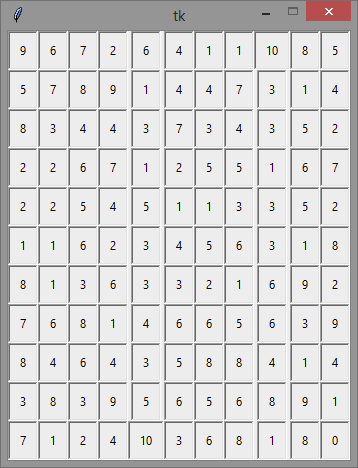
\includegraphics[width = .6\linewidth]{11x11_1_eval_10}
		\caption{Evaluation}
		\label{fig8:sfig2}
	\end{subfigure}
\caption{Solvable 11x11. Value: 10.}
\label{fig:11x11good}
\end{figure}

\begin{figure}[H]
	\begin{subfigure}{.5\textwidth}
		\centering
     		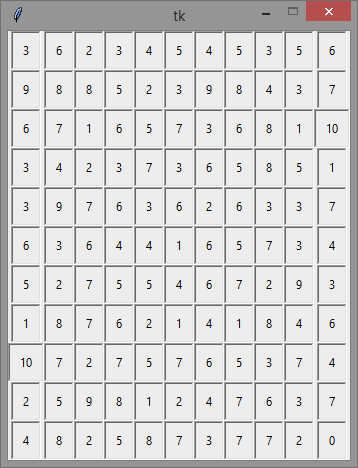
\includegraphics[width = .6\linewidth]{11x11_1_puzzle_-14}
     		\caption{Puzzle}
     		\label{fig9:sfig1}
	\end{subfigure}
	\begin{subfigure}{.5\textwidth}
		\centering
		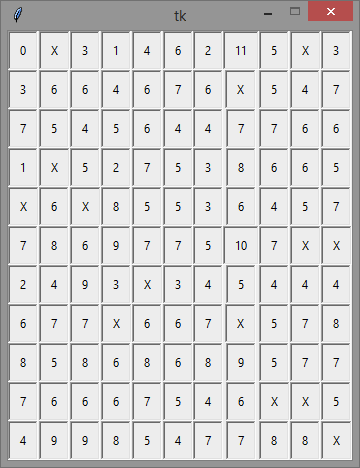
\includegraphics[width = .6\linewidth]{11x11_1_eval_-14}
		\caption{Evaluation}
		\label{fig9:sfig2}
	\end{subfigure}
\caption{Unsolvable 11x11. Value: -14.}
\label{fig:11x11bad}
\end{figure}

\section*{Hill Climbing Approach}

The most basic algorithm we tested was a hill-climbing algorithm. This algorithm randomly changes a tile in the grid. If the new value is greater than or equal to the best value of the grid so far, then the change is kept an the hill-climbing algorithm is repeated. Otherwise, the change is discarded. 

\subsection*{Varying Iteration Number}

To measure the effect of iteration number on the output of the hill climbing algorithm, we compared the average final value of grids of differing sizes with different iteration numbers to see what the optimal number of iterations would be for the different sized grids. We tested average final value averaged over 50 runs for iteration numbers of 1,000; 5,000; 10,000; 15,000; and 20,000 for grids of size 5 by 5, 7 by 7, 9 by 9, and 11 by 11.

\begin{figure}[H]
    \centering
    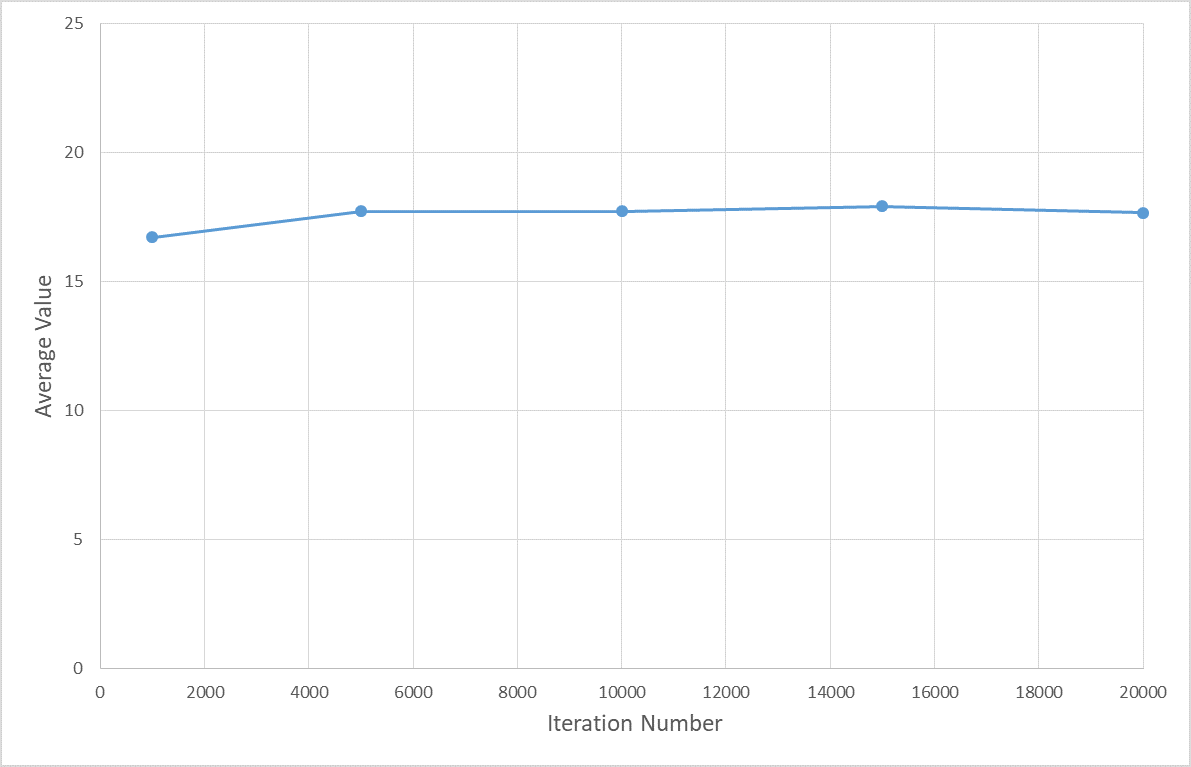
\includegraphics[width=0.9\textwidth]{hill_climbing_5x5_iterations_excel}
\begin{tabular}{ |p{4cm}||p{4cm}|p{4cm}|  }
 \hline
Grid Side Length& Iteration Number &Average Value\\
 \hline
5&1,000&16.72\\
5&5,000&17.72\\
5&10,000&17.72\\
5&15,000&17.92\\
5&20,000&17.66\\
 \hline
\end{tabular}
    \caption{A graph showing the effects of iteration size on final value for a puzzle of size 5 by 5.}
    \label{fig:hill_climbing_5x5_iterations}
\end{figure}

For a 5 by 5 grid, the number of iterations does not seem to make much of a difference, with the largest change being a nominal increase in average value when increasing the iteration number from 1,000 to 5,000. This suggests that the optimal number of iterations that maximizes average value while minimizing computation time is 1,000 iterations for a 5 by 5 grid.

\begin{figure}[H]
    \centering
    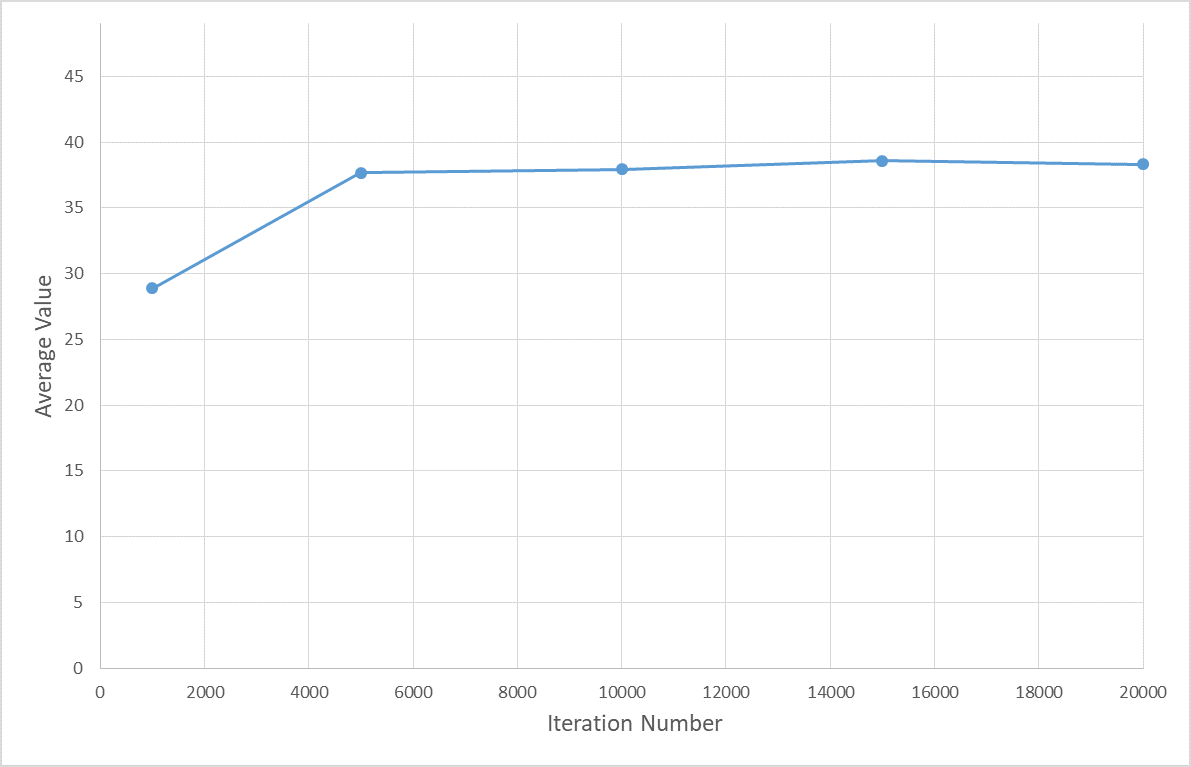
\includegraphics[width=0.9\textwidth]{hill_climbing_7x7_iterations_excel}
\begin{tabular}{ |p{4cm}||p{4cm}|p{4cm}|  }
 \hline
Grid Side Length& Iteration Number &Average Value\\
 \hline
7&1,000&28.88\\
7&5,000&37.66\\
7&10,000&37.94\\
7&15,000&38.58\\
7&20,000&38.30\\
 \hline
\end{tabular}
    \caption{A graph showing the effects of iteration size on final value for a puzzle of size 7 by 7.}
    \label{fig:hill_climbing_7x7_iterations}
\end{figure}

For a 7 by 7 grid, there is a much more marked increase in average value when iteration number increases from 1,000 to 5,000, but once again the average value plateaus as iteration number increases beyond that. This suggests that the optimal number of iterations that maximizes average value while minimizing computation time is 5,000 iterations for a 7 by 7 grid.

\begin{figure}[H]
    \centering
    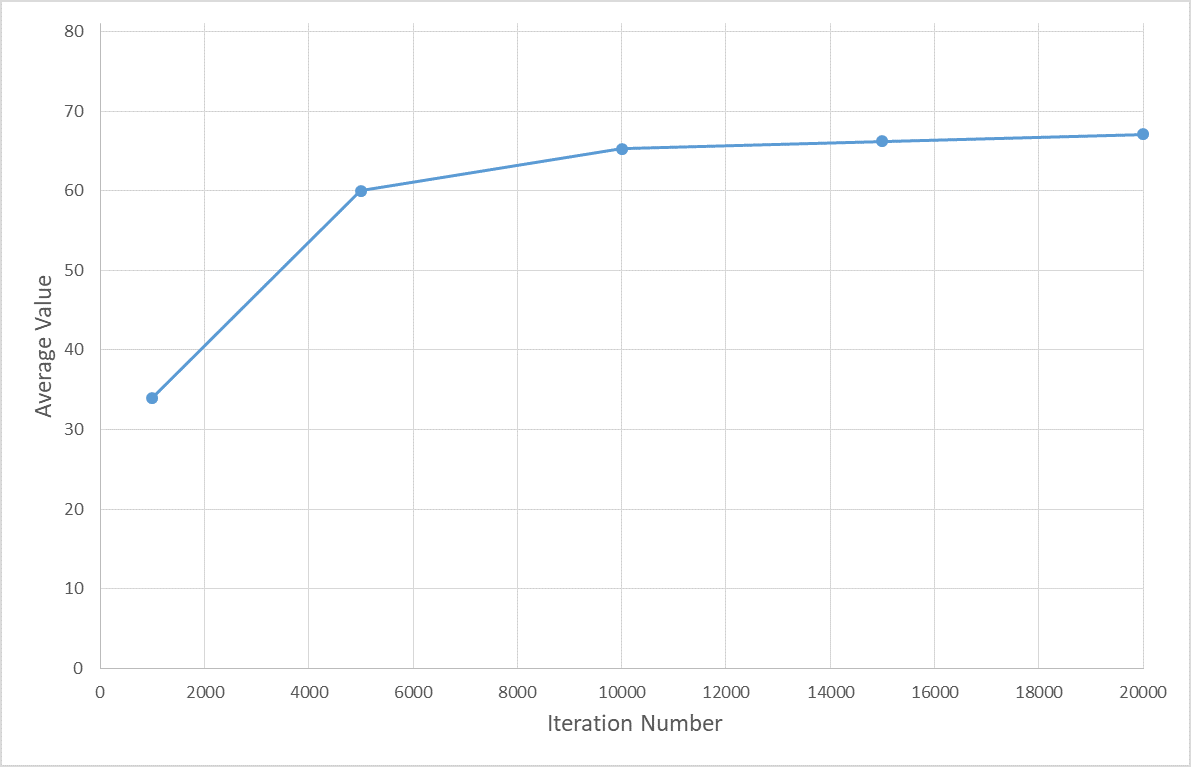
\includegraphics[width=0.9\textwidth]{hill_climbing_9x9_iterations_excel}
\begin{tabular}{ |p{4cm}||p{4cm}|p{4cm}|  }
 \hline
Grid Side Length& Iteration Number &Average Value\\
 \hline
9&1,000&33.96\\
9&5,000&60.02\\
9&10,000&65.30\\
9&15,000&66.24\\
9&20,000&67.10\\
 \hline
\end{tabular}
    \caption{A graph showing the effects of iteration size on final value for a puzzle of size 9 by 9.}
    \label{fig:hill_climbing_9x9_iterations}
\end{figure}

For a 9 by 9 grid, there is a large increase in average value when iteration number increases from 1,000 to 5,000, and another smaller increase when iteration number increases from 5,000 to 10,000. Average value beyond that point increases very slightly. This suggests that the optimal number of iterations that maximizes average value while minimizing computation time is 10,000 iterations for a 9 by 9 grid.

\begin{figure}[H]
    \centering
    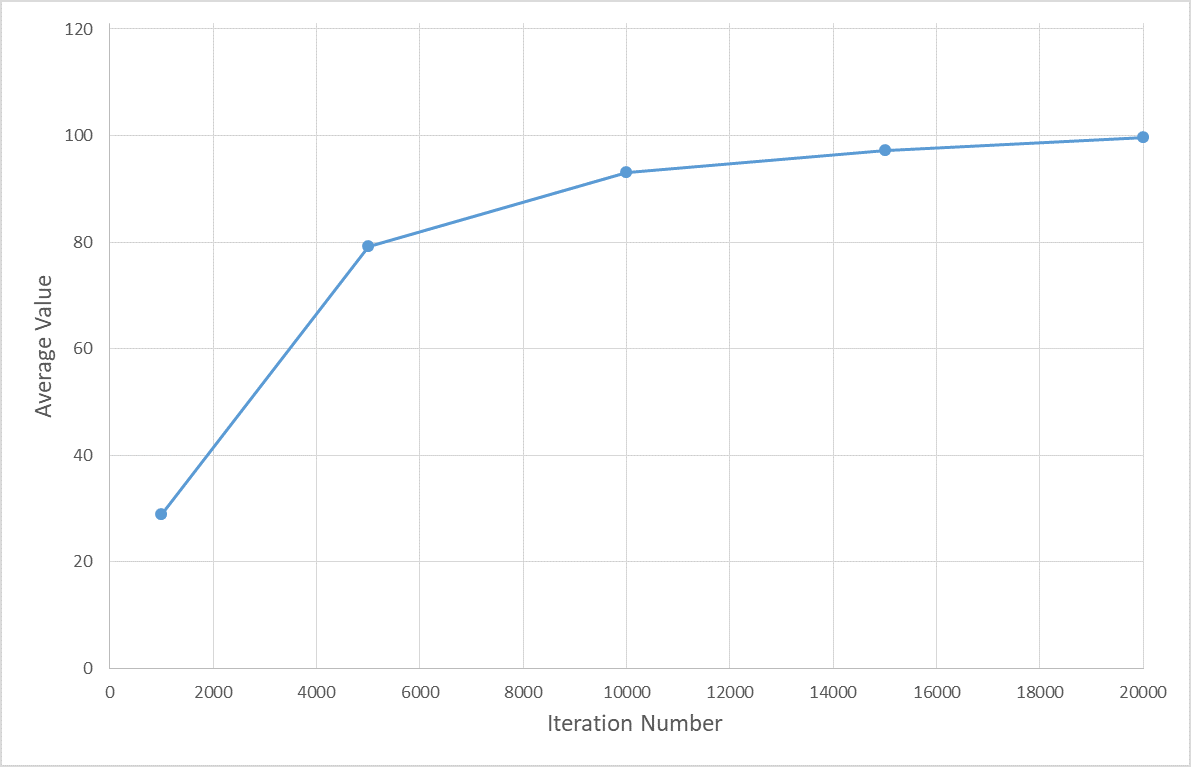
\includegraphics[width=0.9\textwidth]{hill_climbing_11x11_iterations_excel}
\begin{tabular}{ |p{4cm}||p{4cm}|p{4cm}|  }
 \hline
Grid Side Length& Iteration Number &Average Value\\
 \hline
11&1,000&28.86\\
11&5,000&79.20\\
11&10,000&93.08\\
11&15,000&97.28\\
11&20,000&99.66\\
 \hline
\end{tabular}
    \caption{A graph showing the effects of iteration size on final value for a puzzle of size 11 by 11.}
    \label{fig:hill_climbing_11x11_iterations}
\end{figure}



For an 11 by 11 grid, increasing iteration number from 1,000 to 5,000 once again resulted in a steep increase in average value, while subsequent increases in iteration number led to diminishing returns. After 10,000 iterations, subsequent increases in iteration number lead to very small gains. This suggests that the optimal number of iterations that maximizes average value while minimizing computation time is 10,000 iterations for a 11 by 11 grid.


\section*{Hill Climbing with Random Restarts}

The next algorithm we tested was hill-climbing with random restarts. The idea was that a basic hill-climbing algorithm might get stuck at local maxima, where every change would result in a worse grid. In order to circumvent this problem, random restarts would cause the algorithm to start again with a random grid of the same size and run hill-climbing again, repeating the process and keeping track of the best grid.

\subsection*{Varying Restart Number}

All random restart tests were performed with a total of 10,000 iterations. This means that for 2 restarts, there were 5,000 iterations per restart. We tested the effects of having 2, 5, 10, 50, and 100 restarts on grids of size 5 by 5, 7 by 7, 9 by 9, and 11 by 11.

\begin{figure}[H]
    \centering
    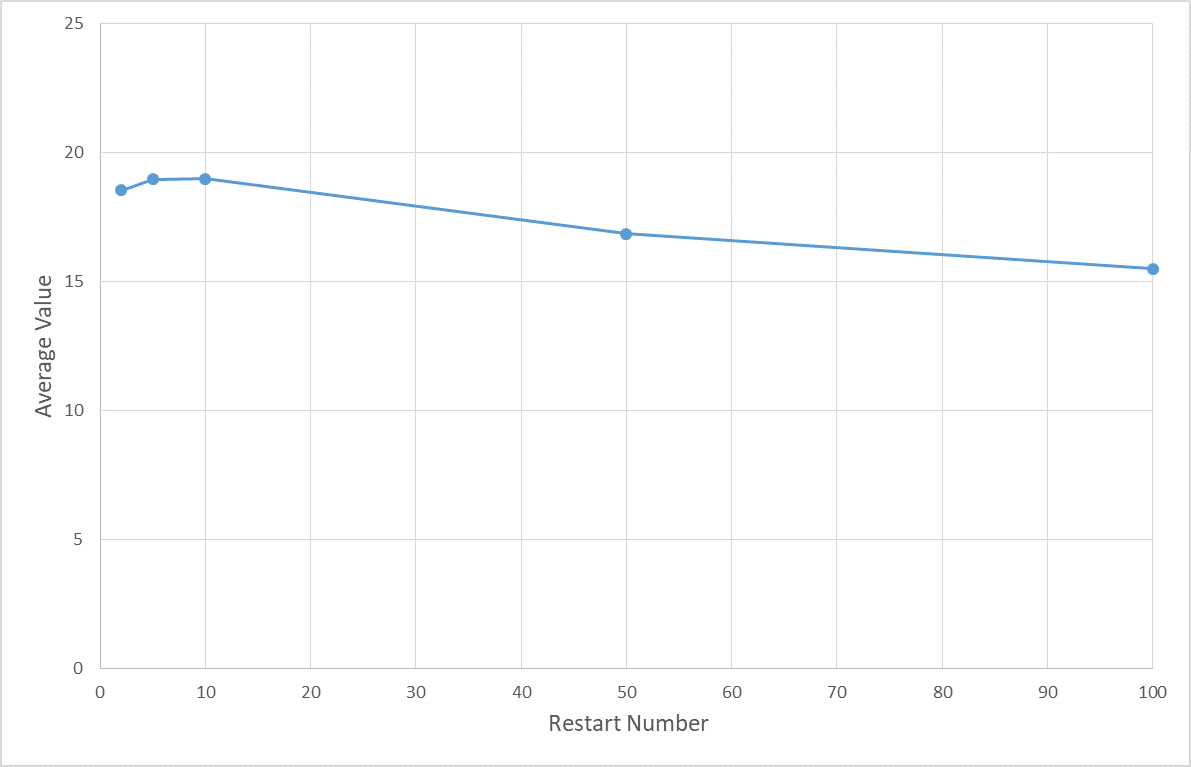
\includegraphics[width=0.9\textwidth]{random_restarts_5x5_restarts_excel}
\begin{tabular}{ |p{4cm}||p{4cm}|p{4cm}|  }
 \hline
Grid Side Length& Restart Number &Average Value\\
 \hline
5&2&18.54\\
5&5&18.96\\
5&10&18.98\\
5&50&16.86\\
5&100&15.50\\
 \hline
\end{tabular}
    \caption{A graph showing the effects of restart number on final value for a puzzle of size 5 by 5.}
    \label{fig:random_restarts_5x5_restarts}
\end{figure}

For a 5 by 5 grid, there is a small increase in average value when restart number increases from 2 to 5, but then average value stays the same until 10 restarts, then plummets. This suggests that the optimal number of restarts for a 5 by 5 grid would be around 2 or 5.

\begin{figure}[H]
    \centering
    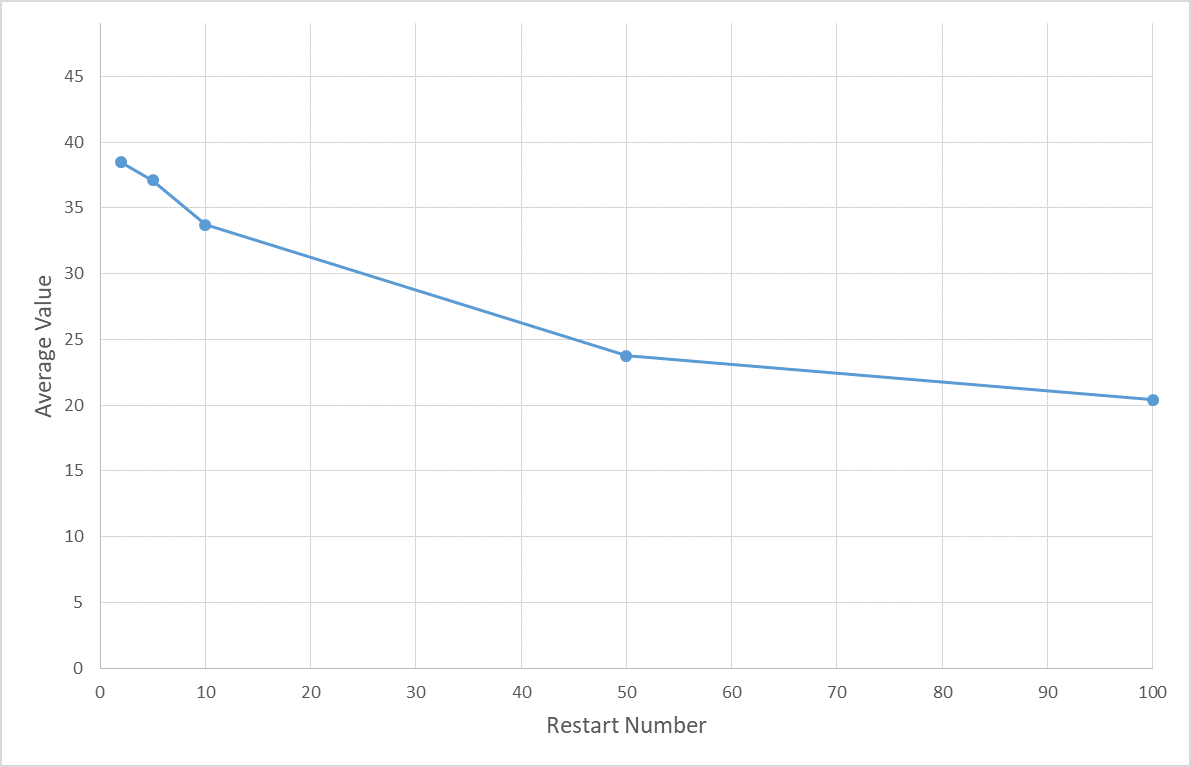
\includegraphics[width=0.9\textwidth]{random_restarts_7x7_restarts_excel}
\begin{tabular}{ |p{4cm}||p{4cm}|p{4cm}|  }
 \hline
Grid Side Length& Restart Number &Average Value\\
 \hline
7&2&38.48\\
7&5&37.08\\
7&10&33.70\\
7&50&23.76\\
7&100&20.40\\
 \hline
\end{tabular}
    \caption{A graph showing the effects of restart number on final value for a puzzle of size 7 by 7.}
    \label{fig:random_restarts_7x7_restarts}
\end{figure}

\begin{figure}[H]
    \centering
    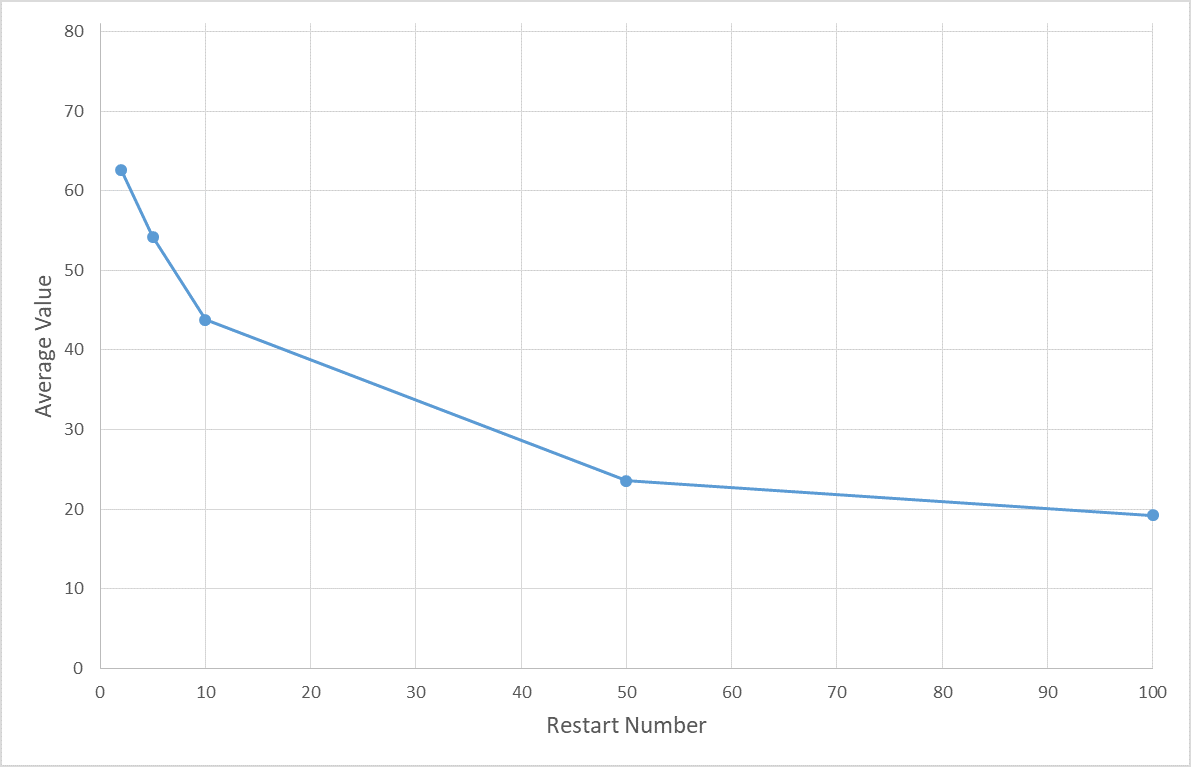
\includegraphics[width=0.9\textwidth]{random_restarts_9x9_restarts_excel}
\begin{tabular}{ |p{4cm}||p{4cm}|p{4cm}|  }
 \hline
Grid Side Length& Restart Number &Average Value\\
 \hline
9&2&62.60\\
9&5&54.20\\
9&10&43.78\\
9&50&23.54\\
9&100&19.22\\
 \hline
\end{tabular}
    \caption{A graph showing the effects of restart number on final value for a puzzle of size 9 by 9.}
    \label{fig:random_restarts_9x9_restarts}
\end{figure}

\begin{figure}[H]
    \centering
    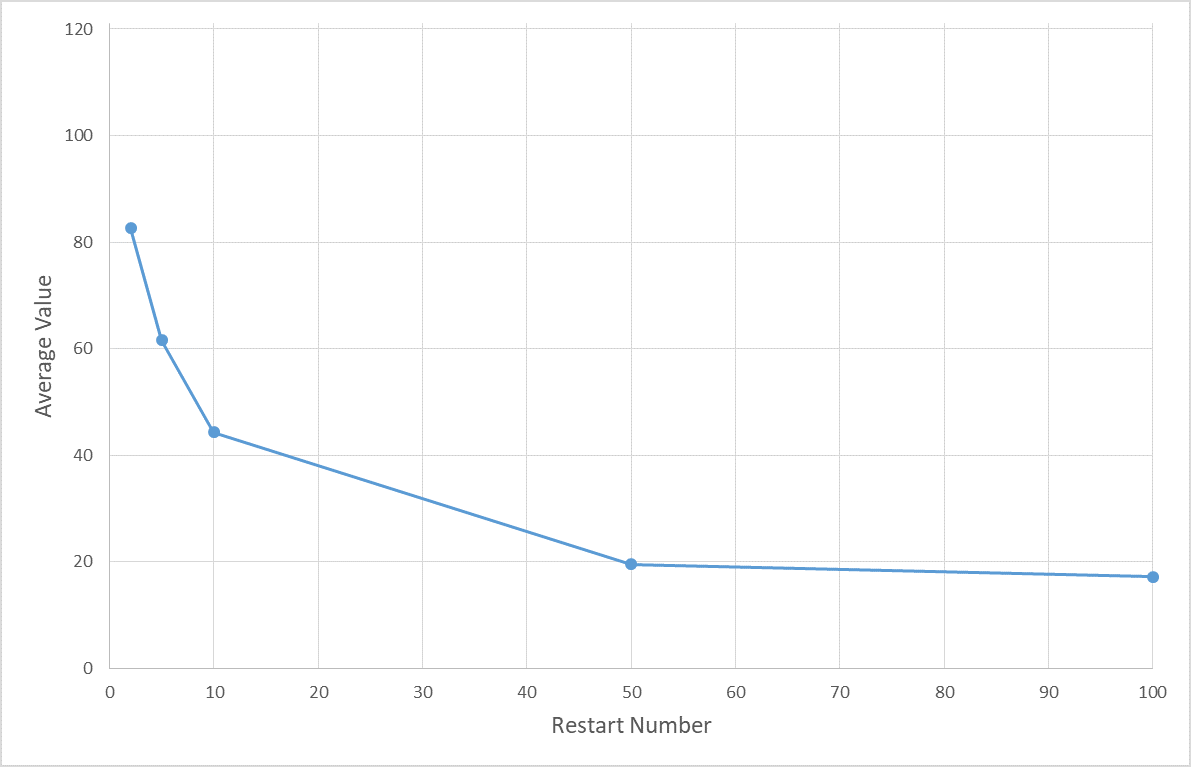
\includegraphics[width=0.9\textwidth]{random_restarts_11x11_restarts_excel}
\begin{tabular}{ |p{4cm}||p{4cm}|p{4cm}|  }
 \hline
Grid Side Length& Restart Number &Average Value\\
 \hline
11&2&82.62\\
11&5&61.60\\
11&10&44.26\\
11&50&19.46\\
11&100&17.16\\
 \hline
\end{tabular}
    \caption{A graph showing the effects of restart number on final value for a puzzle of size 11 by 11.}
    \label{fig:random_restarts_11x11_restarts}
\end{figure}

For grids of larger size, an increase in restart number leads to a decrease in average value, with larger grids leading to a steeper decline. For the hill climbing algorithm, the larger the grid was, the higher the optimal number of iterations was before the average value plateaued. Because an increase from 2 restarts to 5 decreases the number of iterations per restart from 5,000 to just 2,000, this suggests that perhaps there are not enough total iterations for an increase in the number of restarts to outweight the cost of decreasing the number of iterations per restart. For a 5 by 5 grid, which had an optimal iteration number of 1,000, having 5 restarts improved the average value, because having 2,000 iterations per restart was enough to reach the optimal value achievable by a hill climbing algorithm. For an 11 by 11 grid on the other hand, the optimal number of iterations is 10,000, but the total number of iterations run was 10,000. This means that increasing the number of restarts, which decreased the number of iterations per restart, could only decrease the performance of the algorithm for an 11 by 11 grid.

\section*{Hill Climbing with Random Walk}

Another variation of the Hill Climbing algorithm we tested is the Hill Climbing with Random Walk. In order to escapet potential local maxima in the optimization of the puzzles, we adjusted the hill climb to, based on random chance, accept a randomization regardless of the modified graph's evaluation function value. We believed that allowing for reverse walks, in terms of efficiency, would allow more beneficial changes to occur and generate a favorable, final puzzle solution.

\subsection*{Varying Walk Threshold}
As a variation on the Hill Climbing algorithm, Random Walk's main difference is the presence of a condition in which a random probability threshold is used to determine if the algorithm will accept a change regardless if it makes the value better or worse. We examine the effect this addition has on the effectiveness of the algorithm by testing a number of different probabilities over grids of increasing size. \newline

As a note, walk threshold means the likelihood of accepting a change (walking backwards). Zero is equivalent to Hill Climbing. One is purely random.

\begin{figure}[H]
    \centering
    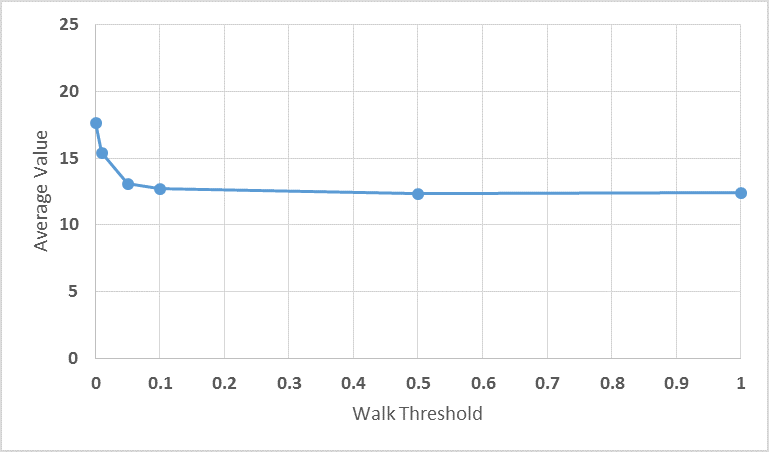
\includegraphics[width=0.9\textwidth]{5x5_RWprob}
\begin{tabular}{ |p{4cm}||p{4cm}|p{4cm}|  }
 \hline
Grid Side Length&Walk Threshold&Average Value\\
 \hline
5&.001&17.62\\
5&.01&15.40\\
5&.05&13.06\\
5&.1&12.70\\
5&.5&12.32\\
5&1&12.40\\
 \hline
\end{tabular}
    \caption{A graph showing the effects of varying Walk probability on a 5x5 grid. 10,000 iterations for each condition}
    \label{fig:RWprob5x5}
\end{figure}

 For the smallest possible grid, there is an exponential decrease in the average value produced by the Random Walk algorithm. The best value is produced at with a probability of .001 which is approximately equivalent to hill climbing performed for an equivalent number of iterations. The average value quickly degenerates to an average value of approximately 12 after two increases to the threshold. The average values appear to follow an exponential decrease over the course of consecutive increases to the walk threshold, and the algorithm performs better at lower thresholds approaching Hill Climbing.
 
\begin{figure}[H]
    \centering
    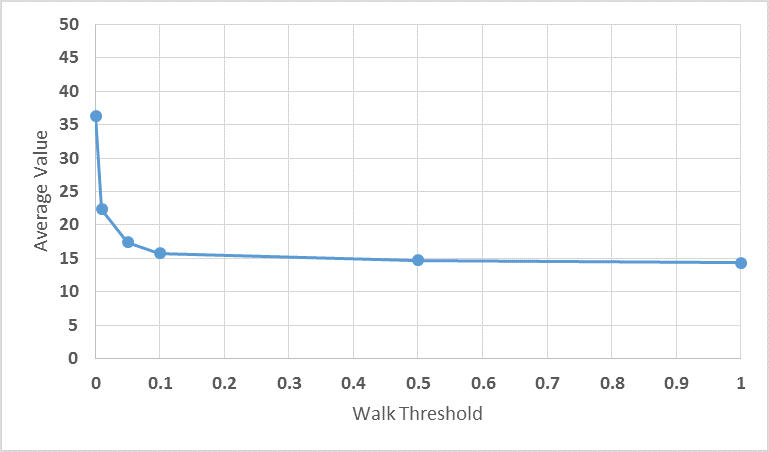
\includegraphics[width=0.9\textwidth]{7x7_RWprob}
\begin{tabular}{ |p{4cm}||p{4cm}|p{4cm}|  }
 \hline
Grid Side Length&Walk Threshold&Average Value\\
 \hline
7&.001&36.28\\
7&.01&22.36\\
7&.05&17.44\\
7&.1&15.78\\
7&.5&14.72\\
7&1&14.38\\
 \hline
\end{tabular}
    \caption{A graph showing the effects of varying probability on a 7x7 grid. 10,000 iterations for each condition}
    \label{fig:RWprob7x7}
\end{figure}
 
 The graphs of 5x5 and 7x7 experience similar trends. Given that the average values are growing with the graphs, the values and curves for these graphs are experience steeper and steeper exponential decreases. By a threshold probability of .1, the 7x7 grid has already effectively approached its lower limit at a value approximately between 14 and 15. Barring insignificant variations, there is no significant variation in the trend observed in the 5x5 grid.
 
 \begin{figure}[H]
    \centering
    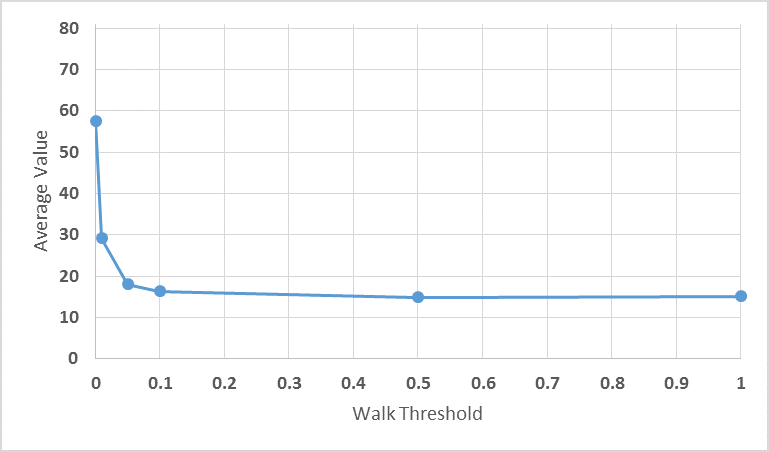
\includegraphics[width=0.9\textwidth]{9x9_RWprob}
\begin{tabular}{ |p{4cm}||p{4cm}|p{4cm}|  }
 \hline
Grid Side Length&Walk Threshold&Average Value\\
 \hline
9&.001&57.46\\
9&.01&29.12\\
9&.05&18.1\\
9&.1&16.36\\
9&.5&14.9\\
9&1&15.12\\
 \hline
\end{tabular}
    \caption{A graph showing the effects of varying probability on a 9x9 grid. 10,000 iterations for each condition}
    \label{fig:RWprob9x9}
\end{figure}
 
As before, the graph of 9x9 has experienced an even more drastic decrease from an average roughly equivalent to Hill Climbing to a lower limit that is apparently the average value of a grid resulting from random changes. However the transition from 7x7 to 9x9 has widened a gap between Random Walk and Hill Climbing at our lowest Walk Threshold. For 10,000 iterations the difference between the average values of a 7x7 grid for Hill Climbing and Random Walk is approximately 1 whereas for a 9x9 grid it is 8. This may be a result of the increase in grid size, but it may also be a deficiency with the Random Walk algorithm. 

 \begin{figure}[H]
    \centering
    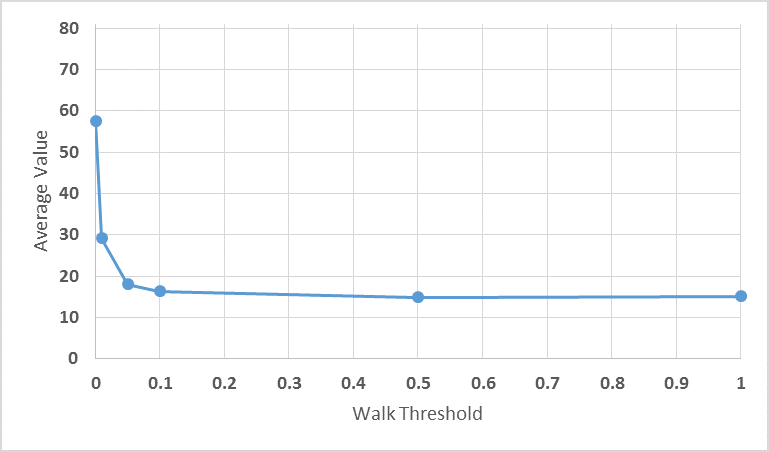
\includegraphics[width=0.9\textwidth]{9x9_RWprob}
\begin{tabular}{ |p{4cm}||p{4cm}|p{4cm}|  }
 \hline
Grid Side Length&Walk Threshold&Average Value\\
 \hline
11&.001&71.28\\
11&.01&32.8\\
11&.05&18.52\\
11&.1&16.42\\
11&.5&14.54\\
11&1&14.24\\
 \hline
\end{tabular}
    \caption{A graph showing the effects of varying probability on a 9x9 grid. 10,000 iterations for each condition}
    \label{fig:RWprob9x9}
\end{figure}

At the largest grid size, the trend remains consistent. As before, the exponential decrease in average value as a result of the intial two threshold probability increases has increased. The lower limit of the average value is again fairly consistent as well. This is notable if only because it represents highlights the effects of the algorithm and illustrates what the average of purely randomized changes can produce as a best puzzle's value across all 4 grid sizes. \newline

Overall, Random Walk seems to perform the best with threshold values approaching zero. It is possible that the average value could be improved over pure Hill Climbing at some probability incredibly close to zero, but this is likely only to be relevant at iteration numbers greatly surpassing 10000. A re-evaluation of threshold probabilities may give a slightly less homogenous curve, though the inverse correlation of average value and walk threshold as the probability approaches 1 is likely to remain consistent. For example, a range of probabilites much closer to zero: .00001, .0001, .001, .01. Due to resource constraints we were unable to perform this analysis.

\section*{Simulated Annealing}

A variation of random walk is known as simulated annealing. While random walk has a fixed probability that an inferior move will be chosen, simulated annealing instead uses the equation

\begin{equation}
e^{\frac{V(J') - V(j)}{T}}
\end{equation}

to calculate the chance that a worse move will be accepted, where V(J') is the value of the current grid, V(j) is the value of the best grid, and T is the temperature. When simulated annealing is run, an initial temperature is given, and it decays at a given rate every time an iteration completes. When temperature is high, negative changes are more likely to be accepted. When temperature is low, negative change are very unlikely to be accepted. We tested the average value of simulated annealing for various values of initial temperature and the decay rate.

\subsection*{Varying Initial Temperature}

All simulated annealing algorithms were run with 10,000 algorithms and a decay rate of 0.99. This means that the initial temperature is multiplied by 0.99 after every iteration.

\begin{figure}[H]
    \centering
    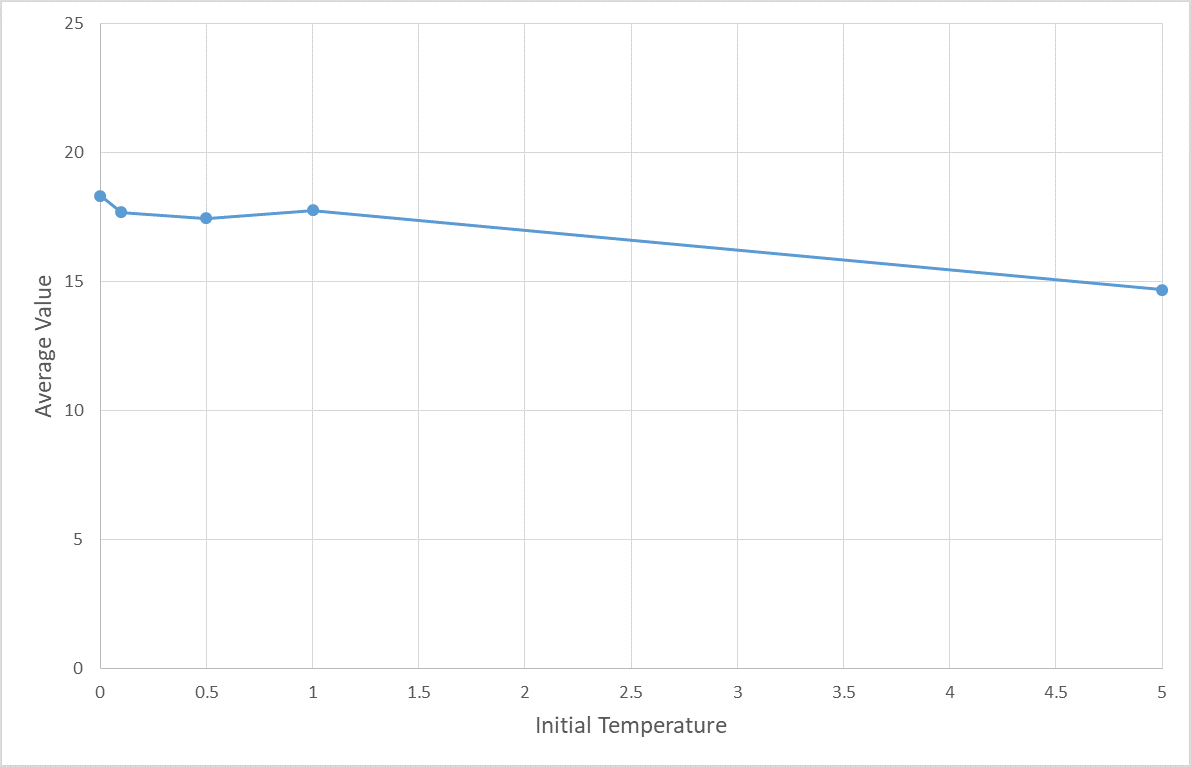
\includegraphics[width=0.9\textwidth]{simulated_annealing_5x5_temperature_excel}
\begin{tabular}{ |p{4cm}||p{4cm}|p{4cm}|  }
 \hline
Grid Side Length& Initial Temperature &Average Value\\
 \hline
5&0&18.32\\
5&0.1&17.68\\
5&0.5&17.46\\
5&1&17.76\\
5&5&14.68\\
 \hline
\end{tabular}
    \caption{A graph showing the effects of initial temperature on final value for a puzzle of size 5 by 5.}
    \label{fig:simulated_annealing_5x5_temperature}
\end{figure}

A larger initial temperature means that more detrimental moves will be accepted overall. In this graph, an initial temperature of 0 actually performs best, with a small decline as temperature increases before average value increases again as temperature reaches 1. Increasing initial temperature to 5 however results in a decrease in average value. This suggests that for smaller grids, a small initial temperature may be preferable. The optimal temperature seems to be 0 or 1.

\begin{figure}[H]
    \centering
    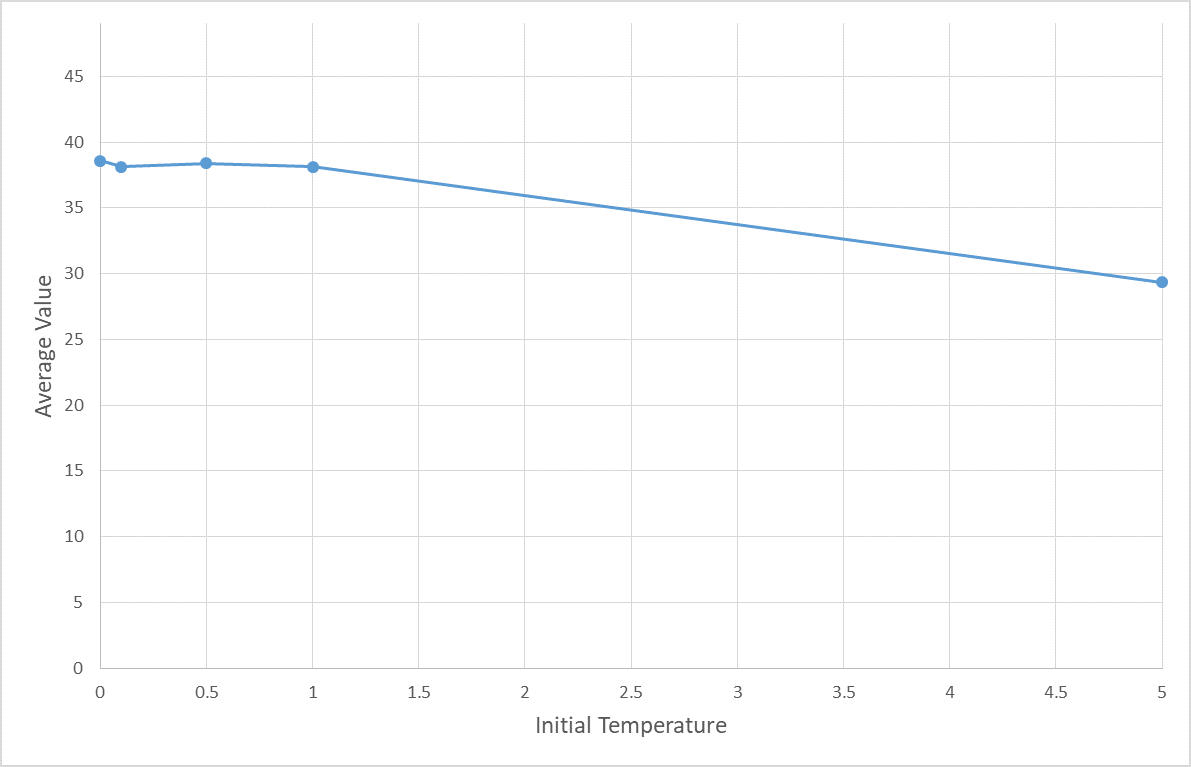
\includegraphics[width=0.9\textwidth]{simulated_annealing_7x7_temperature_excel}
\begin{tabular}{ |p{4cm}||p{4cm}|p{4cm}|  }
 \hline
Grid Side Length& Initial Temperature &Average Value\\
 \hline
7&0&38.56\\
7&0.1&38.12\\
7&0.5&38.38\\
7&1&38.12\\
7&5&29.34\\
 \hline
\end{tabular}
    \caption{A graph showing the effects of initial temperature on final value for a puzzle of size 7 by 7.}
    \label{fig:simulated_annealing_7x7_temperature}
\end{figure}

\begin{figure}[H]
    \centering
    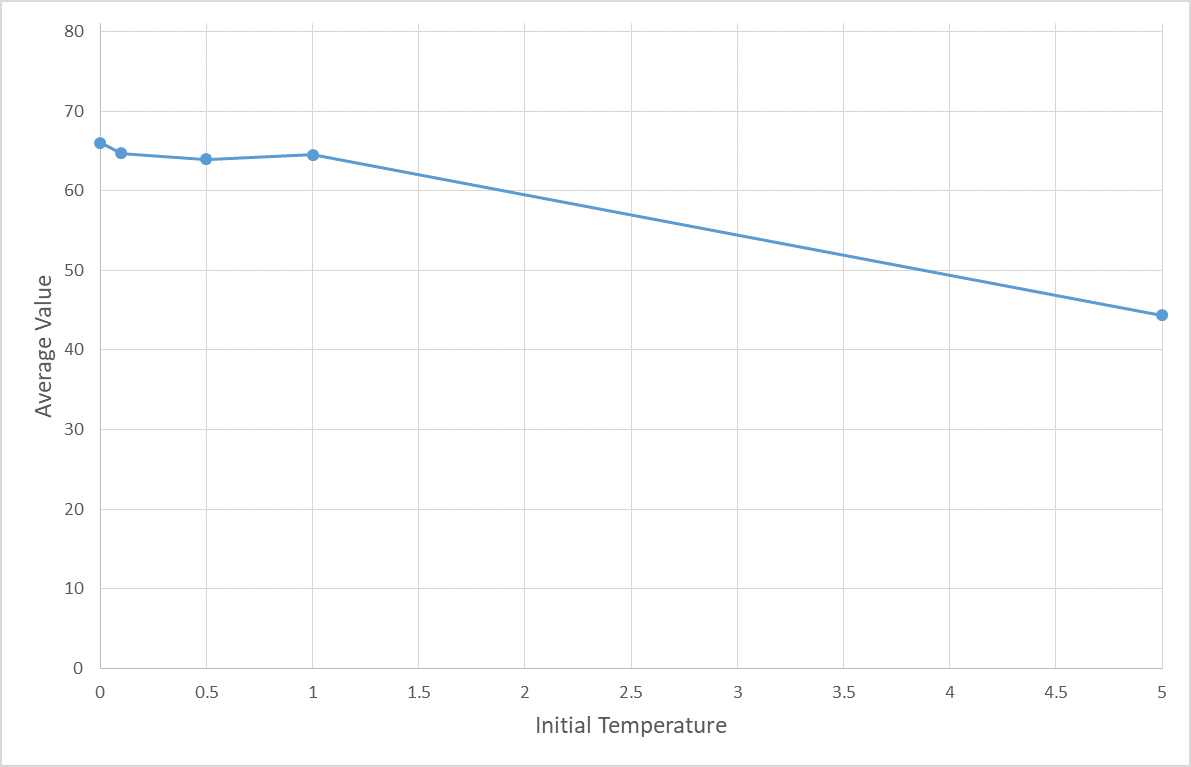
\includegraphics[width=0.9\textwidth]{simulated_annealing_9x9_temperature_excel}
\begin{tabular}{ |p{4cm}||p{4cm}|p{4cm}|  }
 \hline
Grid Side Length& Initial Temperature &Average Value\\
 \hline
9&0&66.04\\
9&0.1&64.72\\
9&0.5&63.96\\
9&1&64.54\\
9&5&44.34\\
 \hline
\end{tabular}
    \caption{A graph showing the effects of initial temperature on final value for a puzzle of size 9 by 9.}
    \label{fig:simulated_annealing_9x9_temperature}
\end{figure}

\begin{figure}[H]
    \centering
    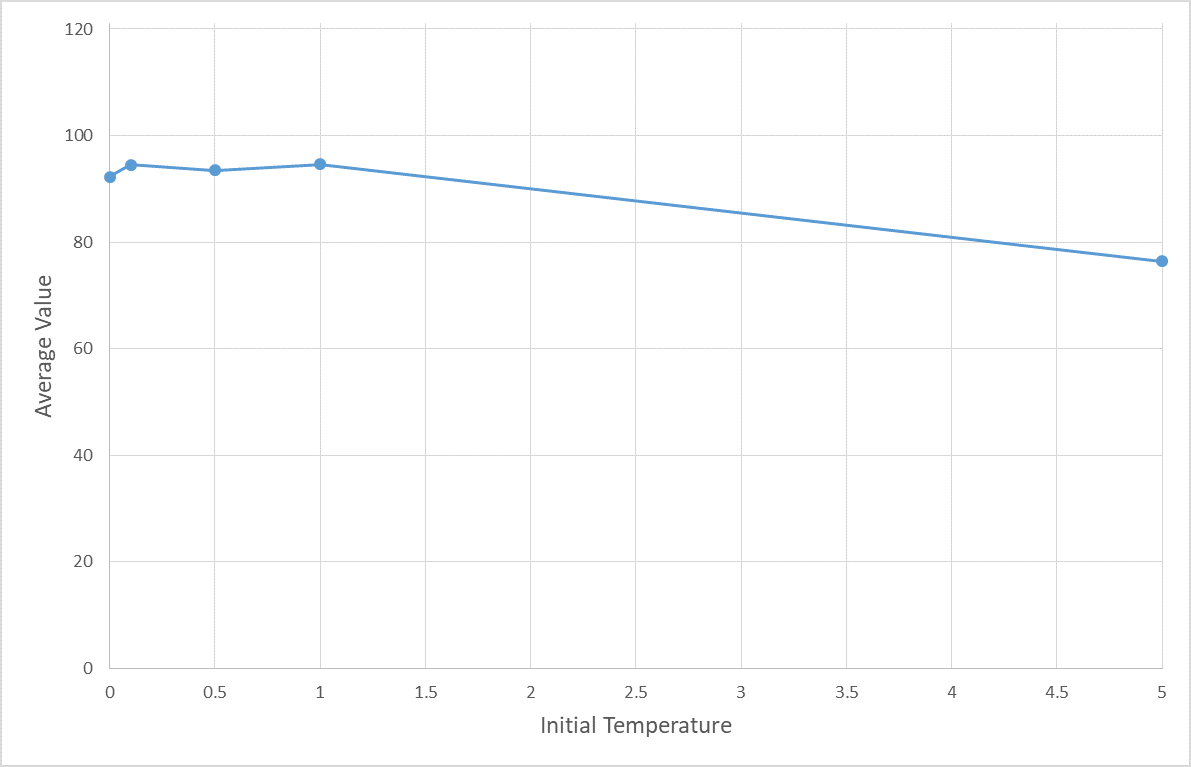
\includegraphics[width=0.9\textwidth]{simulated_annealing_11x11_temperature_excel}
\begin{tabular}{ |p{4cm}||p{4cm}|p{4cm}|  }
 \hline
Grid Side Length& Initial Temperature &Average Value\\
 \hline
11&0&92.24\\
11&0.1&94.48\\
11&0.5&93.44\\
11&1&94.62\\
11&5&76.42\\
 \hline
\end{tabular}
    \caption{A graph showing the effects of initial temperature on final value for a puzzle of size 11 by 11.}
    \label{fig:simulated_annealing_11x11_temperature}
\end{figure}

The same trend seems to hold true for grids of all other sizes, with the average value being highest between initial temperatures of 0 and 1 and then decreasing sharply when initial temperature is increased to 5. 11 is a slight outlier in that its optimal initial temperature is at 1 instead of 0, but all grids showed about constant average value between 0 and 1 before decreasing once initial temperature reached 5. Because an initial temperature of 0 means that the algorithm is essentially just hill climbing, an initial temperature of 1 seems to be optimal if you want to perform simulated annealing. This could be because it is high enough that inferior moves are chosen often enough to escape local maxima, while it is low enough that it doesn't devolve into a random walk.

\subsection*{Varying Decay Rate}

We also investigated changing the decay rate of the function. A lower decay rate means that temperature decreases more quickly, while a decay rate closer to 1 means that temperature decreases more slowly. For the following tests, we used 10,000 iterations and an initial temperature of 1.

\begin{figure}[H]
    \centering
    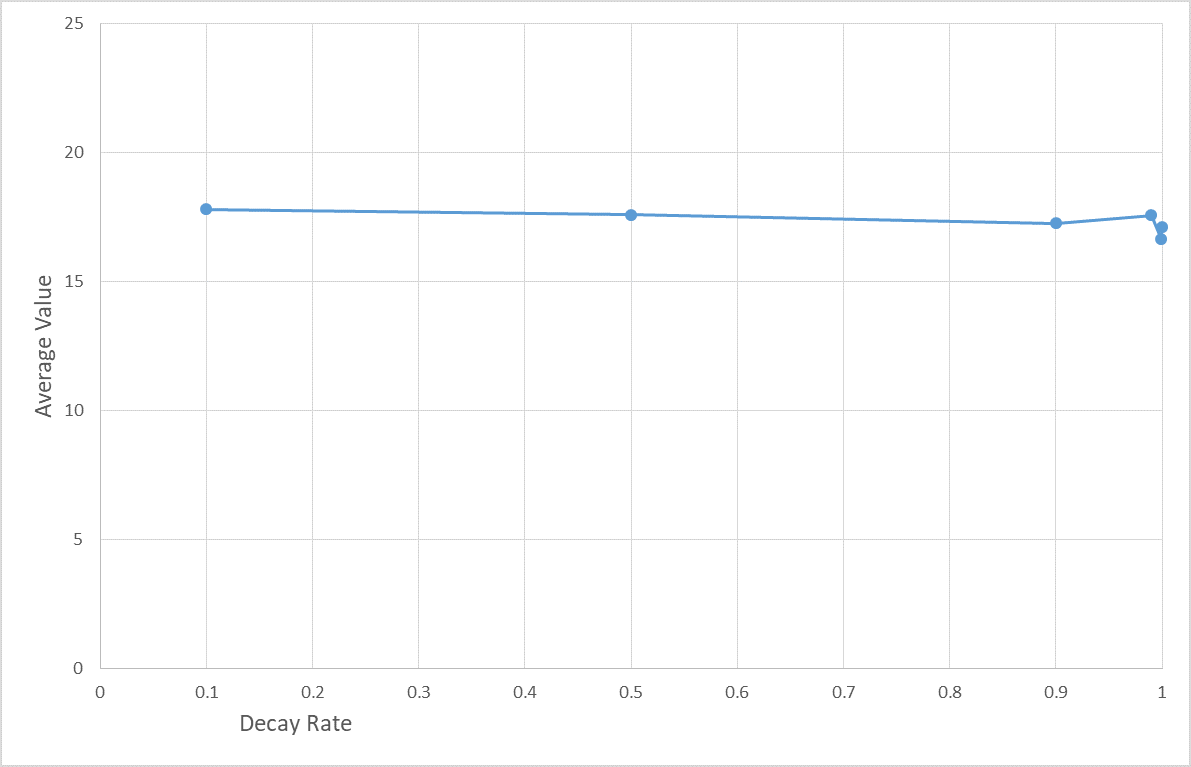
\includegraphics[width=0.9\textwidth]{simulated_annealing_5x5_decay_excel}
\begin{tabular}{ |p{4cm}||p{4cm}|p{4cm}|  }
 \hline
Grid Side Length& Decay Rate &Average Value\\
 \hline
5&0.1&17.80\\
5&0.5&17.58\\
5&0.9&17.26\\
5&0.99&17.56\\
5&0.999&16.64\\
5&1&17.12\\
 \hline
\end{tabular}
    \caption{A graph showing the effects of decay rate on final value for a puzzle of size 5 by 5.}
    \label{fig:simulated_annealing_5x5_decay}
\end{figure}

\begin{figure}[H]
    \centering
    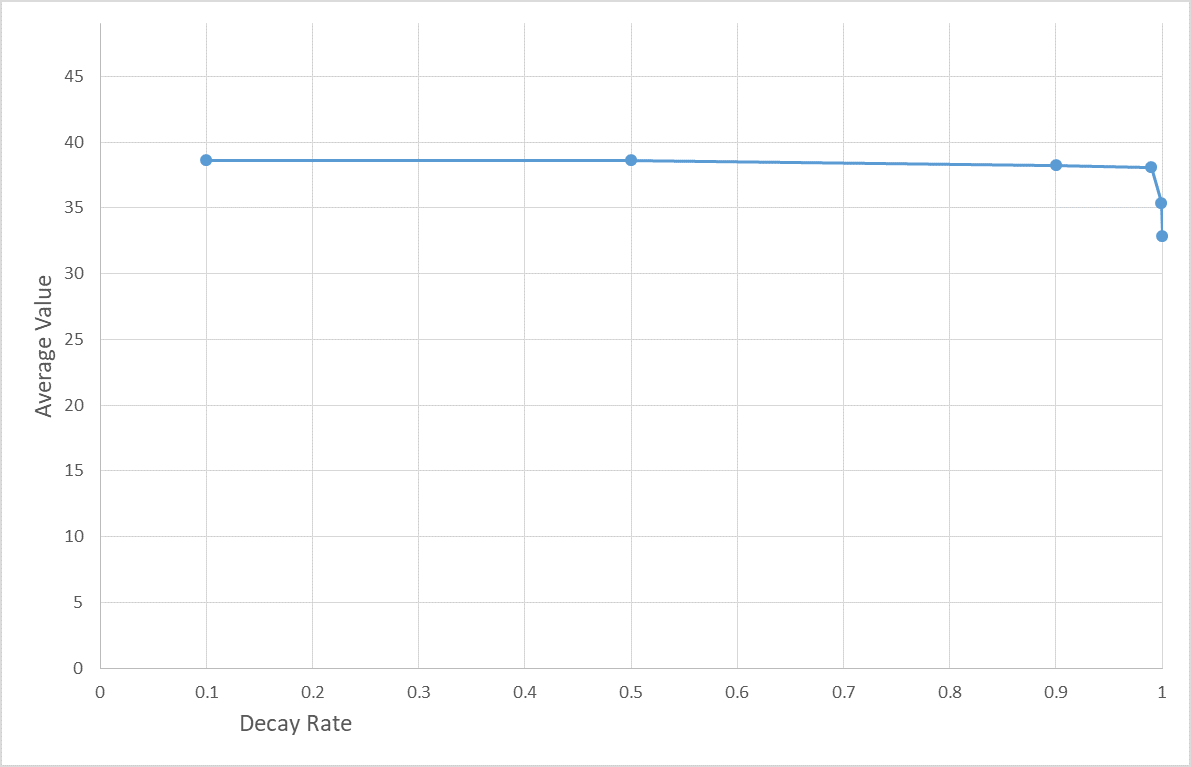
\includegraphics[width=0.9\textwidth]{simulated_annealing_7x7_decay_excel}
\begin{tabular}{ |p{4cm}||p{4cm}|p{4cm}|  }
 \hline
Grid Side Length& Decay Rate &Average Value\\
 \hline
7&0.1&38.60\\
7&0.5&38.62\\
7&0.9&38.24\\
7&0.99&38.08\\
7&0.999&35.38\\
7&1&32.86\\
 \hline
\end{tabular}
    \caption{A graph showing the effects of decay rate on final value for a puzzle of size 7 by 7.}
    \label{fig:simulated_annealing_7x7_decay}
\end{figure}

\begin{figure}[H]
    \centering
    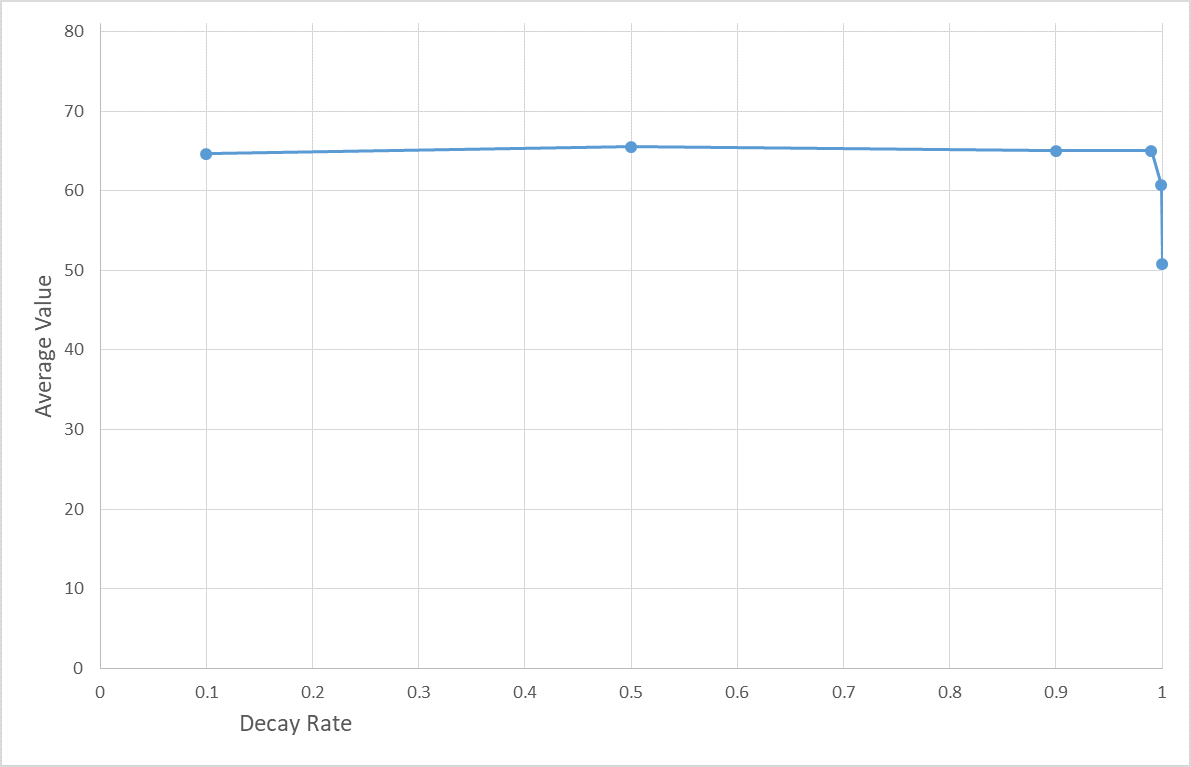
\includegraphics[width=0.9\textwidth]{simulated_annealing_9x9_decay_excel}
\begin{tabular}{ |p{4cm}||p{4cm}|p{4cm}|  }
 \hline
Grid Side Length& Decay Rate &Average Value\\
 \hline
9&0.1&64.64\\
9&0.5&65.60\\
9&0.9&65.00\\
9&0.99&65.04\\
9&0.999&60.70\\
9&1&50.76\\
 \hline
\end{tabular}
    \caption{A graph showing the effects of decay rate on final value for a puzzle of size 9 by 9.}
    \label{fig:simulated_annealing_9x9_decay}
\end{figure}

\begin{figure}[H]
    \centering
    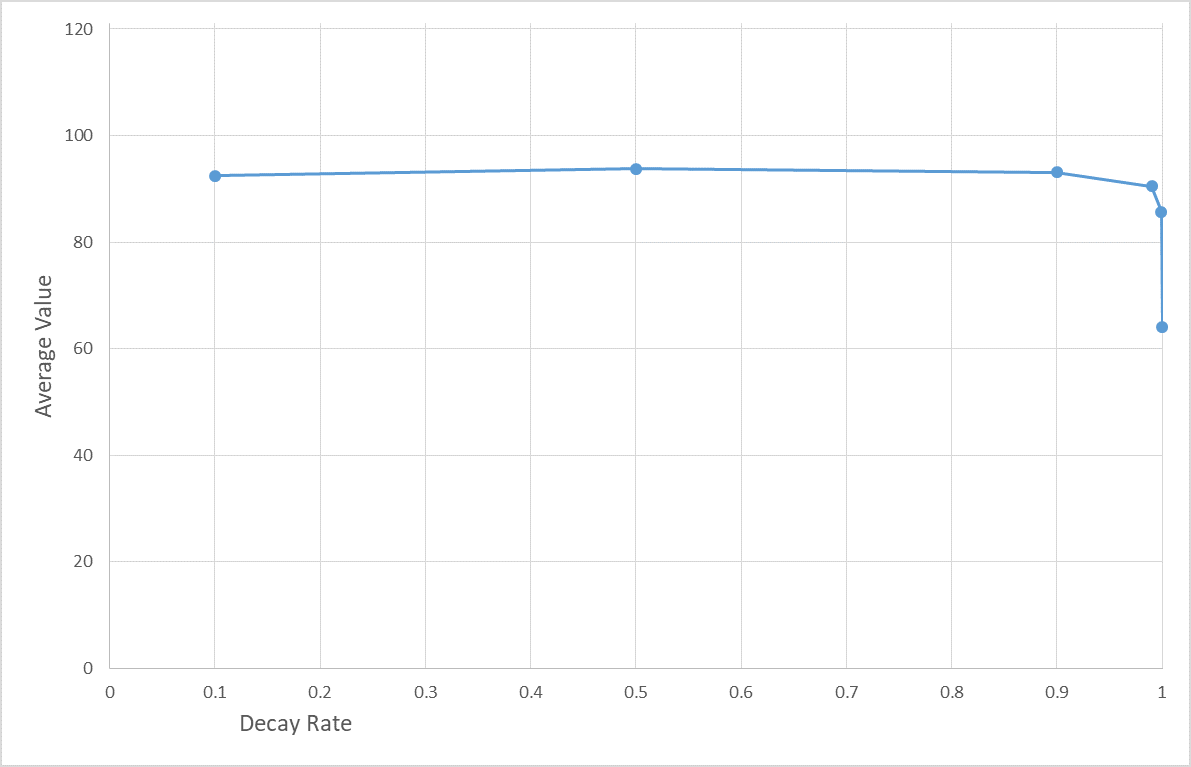
\includegraphics[width=0.9\textwidth]{simulated_annealing_11x11_decay_excel}
\begin{tabular}{ |p{4cm}||p{4cm}|p{4cm}|  }
 \hline
Grid Side Length& Decay Rate &Average Value\\
 \hline
11&0.1&92.40\\
11&0.5&93.80\\
11&0.9&93.08\\
11&0.99&90.52\\
11&0.999&85.66\\
11&1&63.96\\
 \hline
\end{tabular}
    \caption{A graph showing the effects of decay rate on final value for a puzzle of size 11 by 11.}
    \label{fig:simulated_annealing_11x11_decay}
\end{figure}

For all grid sizes, average value seems to increase very gradually as decay rate increases until reaching 0.99, and then average value steeply declines. Because a decay rate of 1 means that the temperature never goes down, this can be explained as the results being too random when decay rate is 1. Average value seems to increase slowly as decay rate increases from 0 to 0.99 because the lower decay rate is, the faster the algorithm devolves into hill climbing. 0.99 seems to be the optimal decay rate, where enough random walking is done at the beginning to escape local maxima while still doing enough hill climbing to maximize the value.

\section*{Genetic Algorithm based upon a Population}

The genetic algorithm we have implemented takes inspiration from the biological principles of natural selection and meitotic cross-over events. Inside a population of graphs, their values are evaluated and set as their fitness values. The probability of each member of the population surviving is assigned by evaluation using their fitness values with a selection algorithm designed to select for maximum fitness inside a population. Using a random number generator, members of the population are selected based upon their assigned probability to progress to the next iteration. Surviving members are then crossed at either a random or pre-determined point in their solution (in this case, their grids) and subsequently randomly mutated to further introduce variation. The cycle is then repeated. \newline

Genetic algorithm is surprisingly, far less effective for an experiment of this nature compared to Hill Climbing and its variants. We find that the reason for this is simply due to the limited size of both population and iterations that can be tested with our hardware.

\subsection*{Selection Probability Equation}
The Selection Probability Equation assigns probabilities based upon the distance a particular member is from the ideal. In this instance, the ideal is the maximum possible moves a puzzle may have or n-squared, if n is the length of one size of a puzzle. The reciprocal of the difference is divided by the total of the population's reciprocals to produce the normalized selection probability. The base probability of each member of a population is represented in the equation (1).

\begin{equation}
\frac{1}{Ideal-Member}
\end{equation}

\subsection*{Varying Population Size}

%5x5
\begin{figure}[H]
    \centering
    \includegraphics[width=0.9\textwidth]{5x5_GA_pop}
\begin{tabular}{ |p{4cm}||p{4cm}|p{4cm}|  }
 \hline
Grid Side Length&Population Size&Average Value\\
 \hline
5&3&12.60\\
5&5&12.86\\
5&10&12.98\\
5&25&12.44\\
5&50&12.50\\
 \hline
\end{tabular}
    \caption{A graph showing the effects of varying population size on a 5x5 grid. 10,000 iterations for each condition. Random Crossover position.}
    \label{fig:GApop5x5}
\end{figure}

%7x7
\begin{figure}[H]
    \centering
    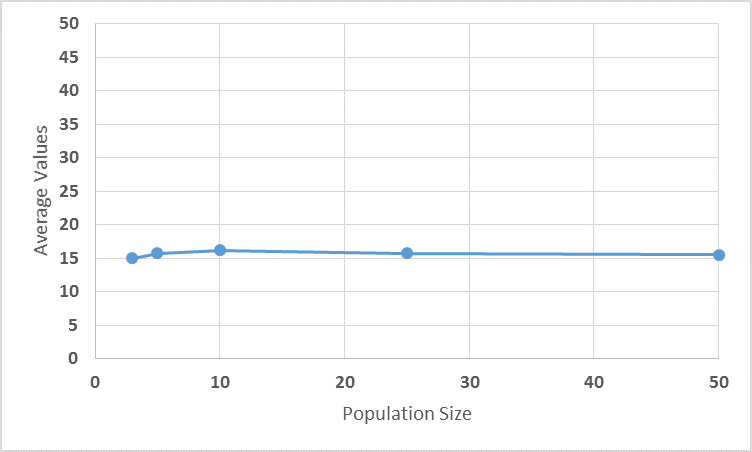
\includegraphics[width=0.9\textwidth]{7x7_GA_pop}
\begin{tabular}{ |p{4cm}||p{4cm}|p{4cm}|  }
 \hline
Grid Side Length&Population Size&Average Value\\
 \hline
7&3&14.94\\
7&5&15.7\\
7&10&16.18\\
7&25&15.72\\
7&50&15.52\\
 \hline
\end{tabular}
    \caption{A graph showing the effects of varying population size on a 7x7 grid. 10,000 iterations for each condition. Random Crossover position.}
    \label{fig:GApop7x7}
\end{figure}

%9x9
\begin{figure}[H]
    \centering
    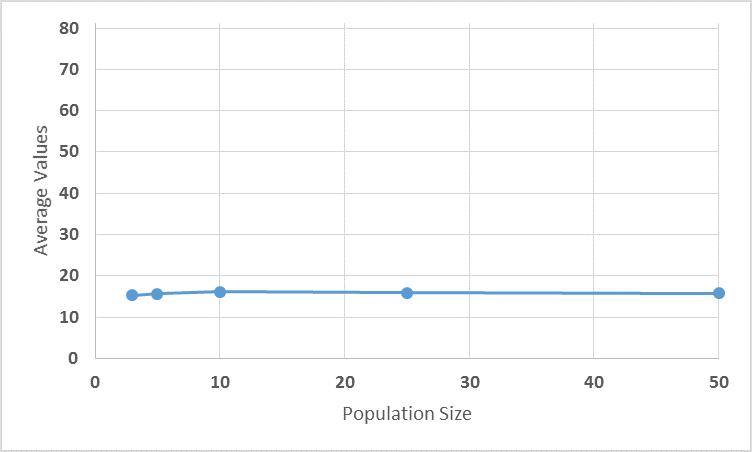
\includegraphics[width=0.9\textwidth]{9x9_GA_pop}
\begin{tabular}{ |p{4cm}||p{4cm}|p{4cm}|  }
 \hline
Grid Side Length&Population Size&Average Value\\
 \hline
9&3&15.28\\
9&5&15.62\\
9&10&16.1\\
9&25&15.95\\
9&50&15.75\\
 \hline
\end{tabular}
    \caption{A graph showing the effects of varying population size on a 7x7 grid. 10,000 iterations for each condition. Random Crossover position.}
    \label{fig:GApop7x7}
\end{figure}

%11x11
\begin{figure}[H]
    \centering
    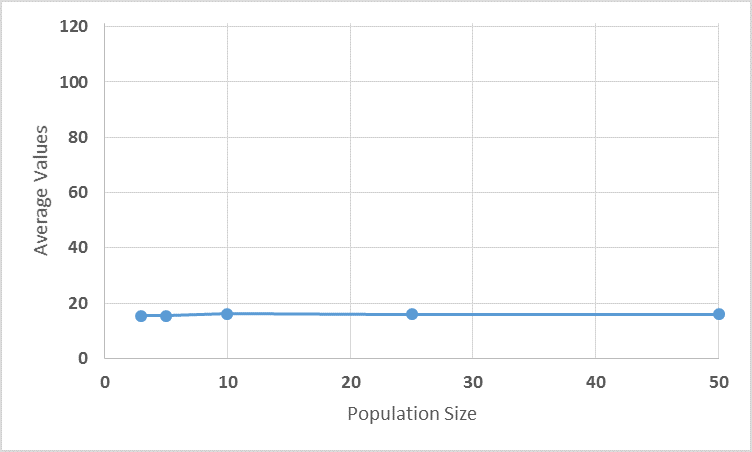
\includegraphics[width=0.9\textwidth]{11x11_GA_pop}
\begin{tabular}{ |p{4cm}||p{4cm}|p{4cm}|  }
 \hline
Grid Side Length&Population Size&Average Value\\
 \hline
11&3&15.42\\
11&5&15.52\\
11&10&16.14\\
11&25&15.90\\
11&50&15.96\\
 \hline
\end{tabular}
    \caption{A graph showing the effects of varying population size on a 11x11 grid. 10,000 iterations for each condition. Random Crossover position.}
    \label{fig:GApop11x11}
\end{figure}

One variable in the genetic algorithm is the population size, or the number of members of a population. This variable has a bearing on the number of available cross overs as well as affecting the relative fitness levels of the members of a population as a result of our selection algorithm. Despite this, the average values of all grid sizes remaints relatively consistent over all population sizes, value roughly between 12 and 17. What this seems to suggest is that despite its theorized effect on the aforementioned properties of the genetic algorithm, population size is negligible in the overall efficiency. 

\subsection*{Varying Crossover Location}

%5x5
\begin{figure}[H]
    \centering
    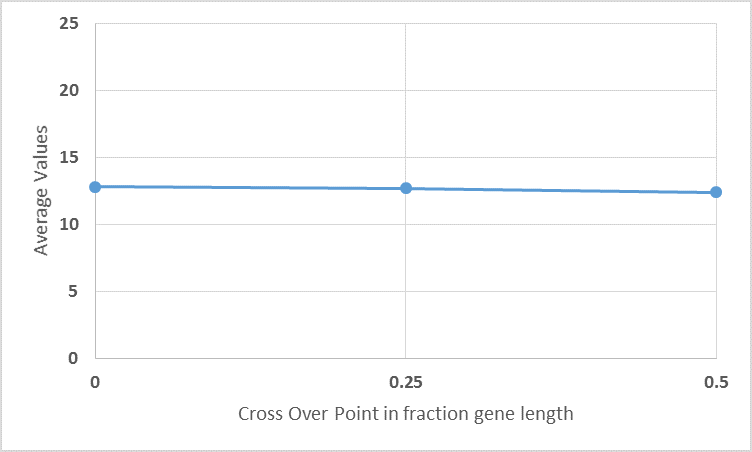
\includegraphics[width=0.9\textwidth]{5x5_GA_Cross}
\begin{tabular}{ |p{4cm}||p{4cm}|p{4cm}|  }
 \hline
Grid Side Length&Crossover Point&Average Value\\
 \hline
5&0&12.84\\
5&.25&12.7\\
5&.50&12.42\\
 \hline
\end{tabular}
    \caption{A graph showing the effects of varying cross over point on a 5x5 grid. 10,000 iterations for each condition. Population size of 5.}
    \label{fig:GAcross5x5}
\end{figure}

%7x7
\begin{figure}[H]
    \centering
    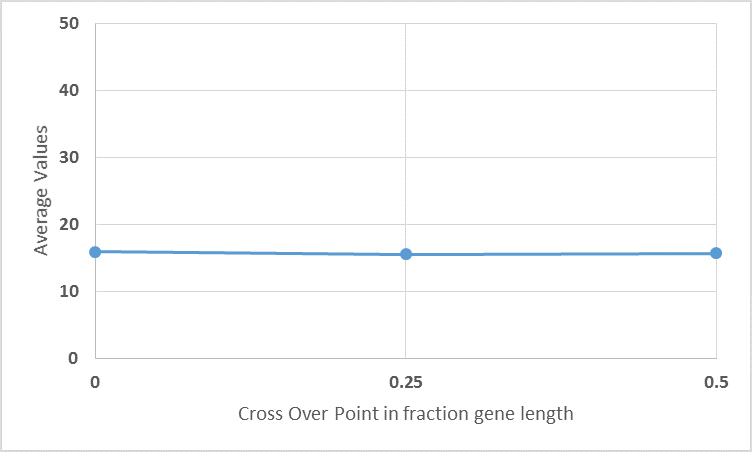
\includegraphics[width=0.9\textwidth]{7x7_GA_Cross}
\begin{tabular}{ |p{4cm}||p{4cm}|p{4cm}|  }
 \hline
Grid Side Length&Crossover Point&Average Value\\
 \hline
7&0&15.92\\
7&.25&15.56\\
7&.50&15.74\\
 \hline
\end{tabular}
    \caption{A graph showing the effects of varying cross over point on a 7x7 grid. 10,000 iterations for each condition. Population size of 5.}
    \label{fig:GAcross7x7}
\end{figure}

%9x9
\begin{figure}[H]
    \centering
    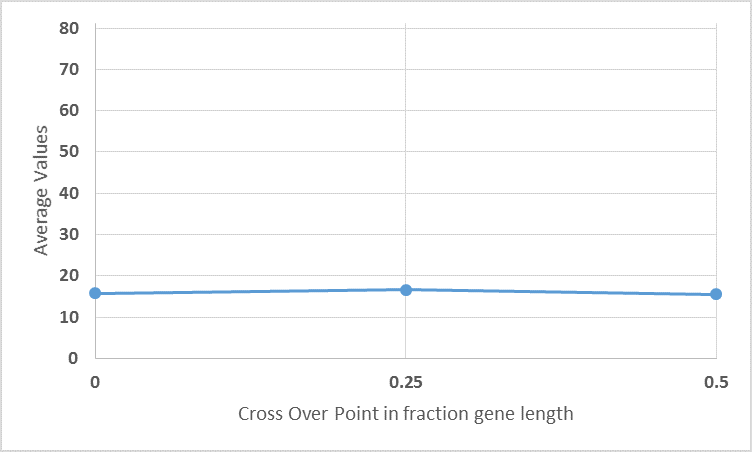
\includegraphics[width=0.9\textwidth]{9x9_GA_cross}
\begin{tabular}{ |p{4cm}||p{4cm}|p{4cm}|  }
 \hline
Grid Side Length&Crossover Point&Average Value\\
 \hline
9&0&15.74\\
9&.25&16.60\\
9&.50&15.52\\
 \hline
\end{tabular}
    \caption{A graph showing the effects of varying cross over point on a 9x9 grid. 10,000 iterations for each condition. Population size of 5.}
    \label{fig:GAcross7x7}
\end{figure}

%11x11
\begin{figure}[H]
    \centering
    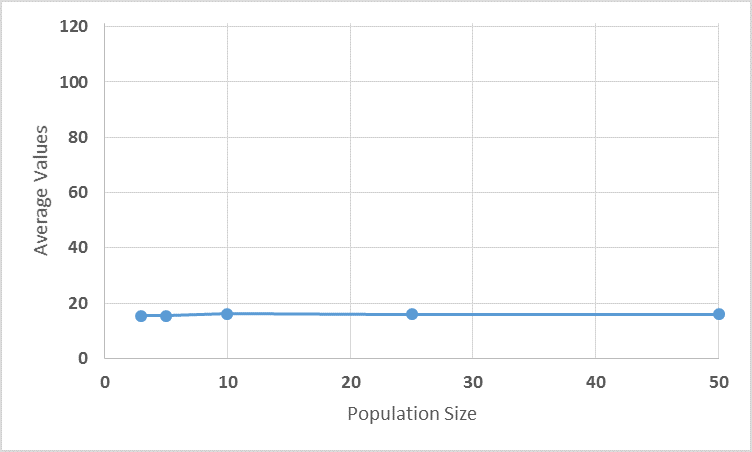
\includegraphics[width=0.9\textwidth]{11x11_GA_pop}
\begin{tabular}{ |p{4cm}||p{4cm}|p{4cm}|  }
 \hline
Grid Side Length&Crossover Point&Average Value\\
 \hline
11&0&15.62\\
11&.25&15.88\\
11&.50&15.86\\
 \hline
\end{tabular}
    \caption{A graph showing the effects of varying cross over point on a 11x11 grid. 10,000 iterations for each condition. Population size of 5.}
    \label{fig:GAcross11x11}
\end{figure}

Crossing over in our algorithm is the swapping of portions of grids based on the location provided on a range of 0 to n-squared, 0 being a simple swap of the members to points representing .25, or one quarter, and .50, or one half, of each member with another member in the population. These notations appear in the tabular data. Members were swapped in a round robin style where, if a population were imagined to be a queue, the swaps would occur with an immediate partner with the ends of the queue wrapping around to complete the cross. \newline

As before, the crossover point seems to be a negligible point of the genetic algorithm with all values approaching a consistent value despite variations in the positioin. This value is roughly between 12 and 17. One of our hypothesized explanations is that the crossing over is indiscriminate and will cross fitter memberes with less fit members despite the contradiction in doing so.

\subsection{Varying Iterations}

%5x5
\begin{figure}[H]
    \centering
    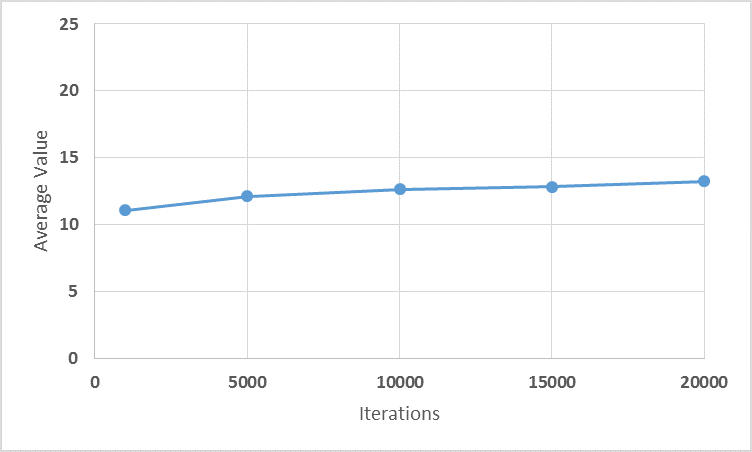
\includegraphics[width=0.9\textwidth]{5x5_GA_Iteration}
\begin{tabular}{ |p{4cm}||p{4cm}|p{4cm}|  }
 \hline
Grid Side Length&Iterations&Average Value\\
 \hline
5&1000&11.08\\
5&5000&12.14\\
5&10000&12.66\\
5&15000&12.82\\
5&20000&13.24\\
 \hline
\end{tabular}
    \caption{A graph showing the effects of varying iterations on a 5x5 grid. Population of 5. Random Crossover position.}
    \label{fig:GApop5x5}
\end{figure}

%7x7
\begin{figure}[H]
    \centering
    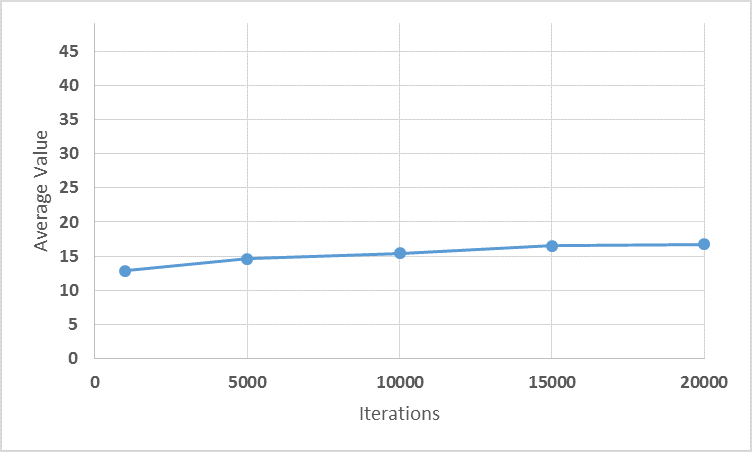
\includegraphics[width=0.9\textwidth]{7x7_GA_Iteration}
\begin{tabular}{ |p{4cm}||p{4cm}|p{4cm}|  }
 \hline
Grid Side Length&Iterations&Average Value\\
 \hline
7&1000&12.84\\
7&5000&14.64\\
7&10000&15.40\\
7&15000&16.52\\
7&20000&16.76\\
 \hline
\end{tabular}
    \caption{A graph showing the effects of varying iterations on a 7x7 grid. Population of 5. Random Crossover position.}
    \label{fig:GApop7x7}
\end{figure}

%9x9
\begin{figure}[H]
    \centering
    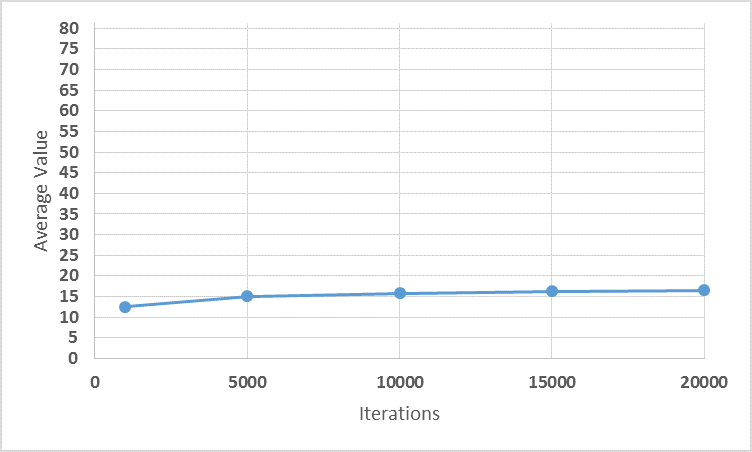
\includegraphics[width=0.9\textwidth]{9x9_GA_Iteration}
\begin{tabular}{ |p{4cm}||p{4cm}|p{4cm}|  }
 \hline
Grid Side Length&Iterations&Average Value\\
 \hline
9&1000&12.56\\
9&5000&15.10\\
9&10000&15.82\\
9&15000&16.34\\
9&20000&16.54\\
 \hline
\end{tabular}
    \caption{A graph showing the effects of varying iterations on a 9x9 grid. Population of 5. Random Crossover position.}
    \label{fig:GApop7x7}
\end{figure}

%11x11
\begin{figure}[H]
    \centering
    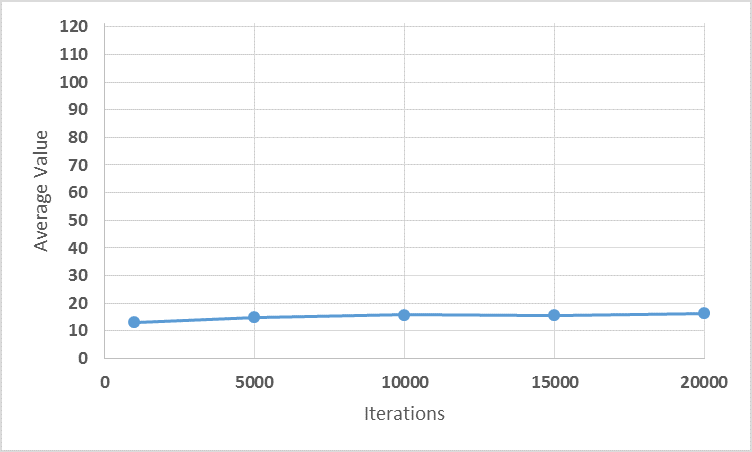
\includegraphics[width=0.9\textwidth]{11x11_GA_Iteration}
\begin{tabular}{ |p{4cm}||p{4cm}|p{4cm}|  }
 \hline
Grid Side Length&Iterations&Average Value\\
 \hline
11&1000&13.1\\
11&5000&14.86\\
11&10000&15.76\\
11&15000&15.70\\
11&20000&16.30\\
 \hline
\end{tabular}
    \caption{A graph showing the effects of varying iterations on a 11x11 grid. Population of 5. Random Crossover position.}
    \label{fig:GApop11x11}
\end{figure}

Given the biological inspiration of the genetic algorithm, another variable worth investigating was iteration number. In an algorithm utilizing some principles of natural selection, undergoing an increasing number of iterations would logically produce a more and more fit population. However, as with the previous two variations, a consistent average value was observed instead. This value was found to be between 12 and 17 as before. We hypothesize this is because of there simply being far too few iterations for the effects to be appreciable, but we are unable to test this hypothesis because of the prohibitively high costs of running more than the provided number of iterations.



\end{document}